%%% Для работы с ГОСТовской рамкой необходимо использовать библиотеку eskdx
%%% Полная документация здесь: https://ctan.org/pkg/eskdx
%%% Выбираем русский язык, кодировку, отображение 26 поля с шифром работы, 
\documentclass[russian, utf8, columnxxvi]{eskdtext}

%%% Языковые пакеты для поддержки русского языка и символов
\usepackage[T1,T2A]{fontenc}
\usepackage[utf8]{inputenc}

%%% Команда, чтобы не нумеровать по звездочке Введение, Заключение и др.
\newcommand*{\No}{\textnumero}

%%% Для оформления ссылок
\usepackage[hidelinks]{hyperref}

%%% Работа с содержанием
\usepackage{tocloft}

%%% Ставим подпись к рисункам. Вместо «рис. 1» будет «Рисунок 1»
\addto{\captionsrussian}{\renewcommand{\figurename}{Рисунок}}

%%% Сложные формулы
\usepackage{amsmath}

%%% Формулы на русском
\usepackage{mathtext}

%%% Умная запятая
\usepackage{icomma}
%%% Автоматически переносить на след. строку слова которые не убираются
%%% в строке
\sloppy

%%% Вставка внешних ПДФ-файлов 
\usepackage[final]{pdfpages}

%%% Для вставки рисунков
\usepackage{graphicx}  % Для вставки рисунков
\graphicspath{{images/}}  % папки с картинками
\setlength\fboxsep{3pt} % Отступ рамки \fbox{} от рисунка
\setlength\fboxrule{1pt} % Толщина линий рамки \fbox{}
\usepackage{wrapfig} % Обтекание рисунков текстом

%%% Для вставки интернет ссылок, полезно в библиографии
\usepackage{url}

%%% Подподразделы(\subsubsection) не выводим в содержании
\setcounter{tocdepth}{2}

%%% Каждый раздел (\section) с новой страницы
\let\stdsection\section
\renewcommand\section{\newpage\stdsection}

%%% Размеры в определенных полях
\renewcommand{\ESKDfontVsize}{\fontsize{15pt}{12pt}}
\renewcommand{\ESKDfontIIIsize}{\fontsize{8pt}{12pt}}

%%% Шрифты
\usepackage{extsizes} % Большие шрифты
\usepackage{upgreek} % Подключение греческого алфавита командами

%%% Подключаем пакет для красивого оформления кода
%%% Можно и lstlisting, но там проблемы с кодировкой
\usepackage{minted}

%%% Переименовываем подпись к листингам
\renewcommand\listingscaption{Листинг}

%%% Библиография
\makeatletter
\renewcommand{\@biblabel}[1]{#1}   % Заменяем библиографию с квадратных скобок на точку
\makeatother

%%% ESKDX %%%

%%% Название документа
\ESKDdocName{\small Название дипломной работы \\ Пояснительная записка}

%%% Разработчик
\ESKDauthor{\tiny Котляревская\,М.\,В.}
%%% Проверяющий
\ESKDchecker{Жиленков\,А.\,А.}
%%% Нормконтроль
\ESKDnormContr{Ведяков\,А.\,А.}
%%% Утверждено
\ESKDapprovedBy{Бобцов\,А.\,А.}

%%% Шифр ПЗ
\ESKDsignature{КСУИ.106.3435.001 ПЗ}

%%% Шифр для перевернутого прямоугольника с шифром на страницах
\ESKDcolumnXXV{КСУИ.106.3435.001 ПЗ}
\ESKDcolumnIX{\small Университет\\
кафедра, группа}

%%% Вертикальные отступы
\ESKDsectSkip{section}{7mm}{7mm}
\ESKDsectSkip{subsection}{5mm}{5mm}

%%% Добавление 26го поля для шифра
\ESKDputOnStyle{formIIab}{columnxxvi}{\ESKDdrawColumnXXVI}
\ESKDsectStyle{section}{\Large\bfseries}
\ESKDsectSkip{section}{8pt}{10pt}
\ESKDsectSkip{subsection}{8pt}{8pt}

%%% Переименовываем библиографию
\addto\captionsrussian{\def\refname{Список использованных источников}}
\usepackage{caption}

%%% Межстрочный интервал
\linespread{1.5}

%%% Для таблиц
\usepackage{array}

%%% Способ ручной установки полей
\usepackage{geometry}
\geometry{top=2.25cm} %поле сверху
\geometry{bottom=2.5cm} %поле снизу
\geometry{left=2.5cm} %поле справа
\geometry{right=1cm} %поле слева

%%% Позволяет рисовать графику 
\usepackage{tikz}
%%% Тоже самое, вдруг понадобится
%\usepackage[texcoord]{eso-pic}

%%% Если перевернутая поле с шифром нужно только на определенной странице легче сделать так
\newcommand\PlaceText[3]{%
\begin{tikzpicture}[remember picture,overlay]
\node[outer sep=0pt,inner sep=0pt,anchor=south west] 
  at ([xshift=#1,yshift=-#2]current page.north west) {#3};
  \draw[line width = 1pt] (9,-0.5) -- (9,-1.9) -- (2,-1.9);
\end{tikzpicture}%
}

%%% Чтобы многостраничное содержание не нумеровалось
\tocloftpagestyle{empty}

\begin{document}

%%% Вставляем постранично титульный лист
\thispagestyle{empty}
\ESKDthisStyle{empty}

\includepdf[pages=1]{titul.pdf}
\thispagestyle{empty}
\ESKDthisStyle{empty}

\includepdf[pages=2]{titul.pdf}

%%% Устанавливаем глубину, которая определяет какие разделы будут выводиться в содержании
%%% 4 означает, что до подподразделов
\setcounter{secnumdepth}{4}
\thispagestyle{empty}

%%% Устанавливаем с какой страницы считать нумерацию в рамке
\setcounter{page}{4}

%%% Стиль страницы
\ESKDthisStyle{formII}

%%% Содержание по центру
\begin{center}
   \tableofcontents 
\end{center}

%%% Звездочка означает отсутствие нумерации у раздела
\section*{Введение}
\addcontentsline{toc}{section}{Введение}
Тут будет Введение без нумерации.

Пример сложной формулы (\ref{eq:1}).
\begin{equation}
    \label{eq:1}
    \text{если } \nu \geq \text{30 мВ, тогда} 
    \begin{cases}
        \nu \gets c\\
        \upsilon \gets \upsilon + d,
 \end{cases}   
\end{equation}
где $\nu$ и $\upsilon$ являются безразмерными величинами, $a, b, c$ - также безразмерные параметры, $' = d/dt$, где $t$ - это время.

\section{Тут будет моя работа}
Вставим таблицу \ref{table:1}:
%%% Таблицы рекомендую рисовать тут: https://www.tablesgenerator.com/ и вставлять готовую таблицу сюда
\begin{table}[h!]
\caption{Здесь будет подпись к моей таблице}
\label{table:1}
\centering
\begin{tabular}{|l|c|c|}
\hline
\begin{tabular}[c]{@{}c@{}}Модель/\\Параметр\end{tabular} & LIF модель & \begin{tabular}[c]{@{}c@{}}модель \\ Ижикевича\end{tabular} \\ \hline
Биофизическая достоверность                                & $-$        & $-$                                                         \\ \hline
Фаза спайка                                                & $-$        & $+$                                                         \\ \hline
Адаптация импульсов                                        & $+$        & $+$                                                         \\ \hline
Задержка выходного сигнала                                 & $-$        & $+$                                                         \\ \hline
Следовые потенциалы                                        & $-$        & $+$                                                         \\ \hline
Резонатор                                                  & $-$        & $+$                                                         \\ \hline
Интегратор                                                 & $+$        & $+$                                                         \\ \hline
Скачок импульса                                            & $-$        & $+$                                                         \\ \hline
Два режима восстановления                                  & $-$        & $+$                                                         \\ \hline
FLOPS                                                      & 10         & 13                                                          \\ \hline
\end{tabular}
\end{table}

\section{Результаты моей работы}
\begin{figure}[!h]
	\centering
	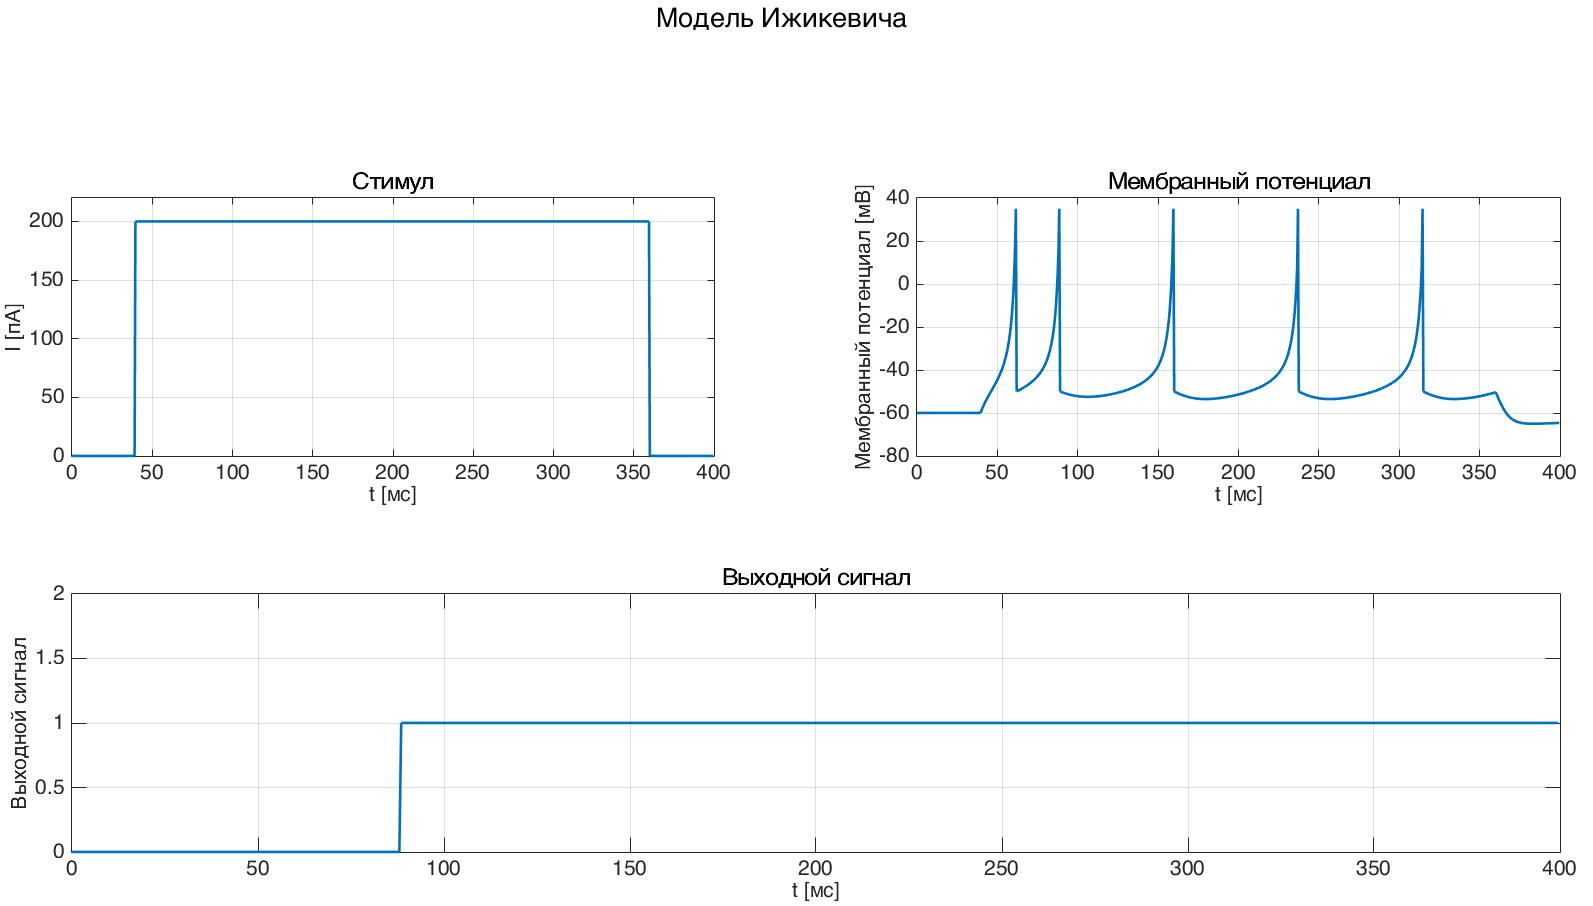
\includegraphics[width=\textwidth]{img/image_1.png}
	\caption{ Какая-то картинка и к ней ссылке в библиографии \cite{art:1}}
	\label{im:1}
\end{figure} 
\section*{Заключение}
\addcontentsline{toc}{section}{Заключение}
Заключение без нумерации будет выглядеть так.

%%% Вставляем библиографию
%%% Определяем стиль библиографии (можно загрузить свой)
\bibliographystyle{gost780u}
%%% Указываем файл с библиографией (должен находиться в той же папке, расширение .bib)
%%% В example_bibliography.bib можно посмотреть атрибуты для каждого типа источника
%%% Использование библиографии: https://ru.sharelatex.com/learn/Bibliography_management_in_LaTeX
\bibliography{rpz}

\ESKDappendix{справочное}{Пример приложения}
%%% Для подписи используем обертку в виде listing, также можно вставлять из файла.
%%% https://ru.sharelatex.com/learn/Code_Highlighting_with_minted
\begin{listing}
    \begin{minted}
    [frame=lines, 
    framesep=2mm, 
    baselinestretch=1.2, 
    fontsize=\small]
    {matlab}
    % Решение прямым методом Эйлера
    for m = 1:NT-1  
        vT     = v(m)+ (dt/2) * (k*(v(m) - vr)*(v(m) - vt)-u(m) + S(m))/C;
        v(m+1) = vT + (dt/2)  * (k*(v(m) - vr)*(v(m) - vt)-u(m) + S(m))/C;
        u(m+1) = u(m) + dt * a*(b*(v(m+1)-vr)-u(m));
        if v(m+1)>= vPeak  % условие появления спайка
           v(m)   = vPeak; % Амплитуда спайкового сигнала
           v(m+1) = c; % сброс мембранного потенциала
           u(m+1) = u(m+1) + d; % обновление переменной восстановления
        end; end;      
    \end{minted}
	\caption{Название листинга}
	\label{lst:1}
\end{listing}
%%% Приложение может быть обязательное, рекомендуемое или справочное
\ESKDappendix{обязательное}{Пример приложения}
\inputminted[frame=lines, framesep=2mm, baselinestretch=1.2, fontsize=\small]{python}{codes/code_2.py}
\end{document}
   

